\documentclass[11pt,a4paper]{article}

\usepackage[T1]{fontenc}
\usepackage[utf8]{inputenc}
\usepackage[brazil]{babel}
\usepackage{lmodern}
\usepackage{amsmath,amssymb}
\usepackage{geometry}
\usepackage{booktabs}
\usepackage{listings}
\usepackage{xcolor}
\usepackage{hyperref}
\usepackage{enumitem}
\usepackage{microtype}
\usepackage{titlesec}
\usepackage{float}
\usepackage{graphicx}

\geometry{margin=2cm}
\titlespacing*{\section}{0pt}{2.0ex plus .4ex minus .2ex}{1.0ex}
\titlespacing*{\subsection}{0pt}{1.5ex plus .3ex minus .2ex}{0.7ex}
\hypersetup{colorlinks=true,linkcolor=black,urlcolor=blue,citecolor=black}
\setlist{nosep}
\setlength{\emergencystretch}{2em}
\lstset{
  basicstyle=\ttfamily\small,
  columns=fullflexible,
  keepspaces=true,
  frame=single,
  breaklines=true,
  showstringspaces=false
}

\title{NERD - BD -- Etapa 2\\\large Pipeline de operadores no modelo materializado: SCAN, FILTER, PROJECT e AGGREGATE}
\author{Rafael Lima Dias\\Projeto de extensão NERD - BD (Banco de Dados)}
\date{Novembro de 2026}

\begin{document}
\maketitle

\begin{abstract}
Este relatório descreve a etapa 2 do motor de consultas didático do Grupo A, escrito em C11 e baseado no modelo de execução materializado. Nesse modelo, cada operador consome a relação de entrada inteira e produz uma tabela de saída completa e independente antes que o operador seguinte comece. São apresentados o pipeline SCAN $\rightarrow$ FILTER $\rightarrow$ PROJECT $\rightarrow$ AGGREGATE, a projeção de colunas, as agregações \texttt{COUNT}, \texttt{SUM}, \texttt{MIN}, \texttt{MAX} e \texttt{AVG}, as regras de alocação e liberação de memória e a validação com o Valgrind. A execução registrada da suíte de testes terminou com 81 alocações, 81 liberações, nenhum vazamento e nenhum erro. O relatório também traz a arquitetura, o fluxograma, as dificuldades encontradas e possíveis otimizações.
\end{abstract}

\section{Introdução}
Um plano de consulta pode ser executado de duas formas principais. No modelo \emph{pipeline} (ou iterador), as tuplas passam de um operador para o outro à medida que são produzidas. No modelo \emph{materializado}, cada operador executa até o fim e grava todo o seu resultado em uma relação temporária, que é então lida pelo operador seguinte \cite{graefe,garcia}. O Grupo A implementa o segundo modelo.

A implementação não possui parser SQL. A consulta é montada no próprio código, encadeando chamadas de função e passando os nomes das colunas como argumentos. A consulta de referência desta etapa é
\par\medskip\noindent\begin{minipage}{\linewidth}
\begin{lstlisting}[language=SQL]
SELECT AVG(salary)
FROM (SELECT id, salary FROM funcionarios WHERE salary > 5000);
\end{lstlisting}
\end{minipage}\par\medskip
que corresponde ao exemplo do enunciado \texttt{SELECT id, salario WHERE salario > 5000}, seguido de uma agregação. No código as colunas têm nomes em inglês (\texttt{id}, \texttt{department}, \texttt{salary}, \texttt{age}). O cabeçalho do CSV, em português (\texttt{id,departamento,salario,idade}), é ignorado na leitura, e os campos são interpretados pela ordem do esquema.

\section{Arquitetura}

\subsection{Módulos}
A Tabela~\ref{tab:modulos} resume a organização do código. Os arquivos \texttt{src/join.c} e \texttt{src/group\_by.c} pertencem à etapa 3 e não são tratados aqui.

\begin{table}[H]
\centering
\small
\begin{tabular}{@{}p{5.3cm}p{11.1cm}@{}}
\toprule
Arquivo & Responsabilidade \\
\midrule
\texttt{include/table.h}, \texttt{src/table.c} & Modelo de dados (\texttt{Schema}, \texttt{Value}, \texttt{Row}, \texttt{Table}), vetor dinâmico de linhas e leitura de CSV tipada pelo esquema \\
\texttt{include/materialized.h} & API dos operadores, \texttt{QueryMetrics}, \texttt{Comparison}, \texttt{AggregateFunction}, \texttt{AggregateResult} \\
\texttt{src/scan.c} & \texttt{materialized\_scan} \\
\texttt{src/materialized.c} & \texttt{materialized\_filter}, \texttt{materialized\_filter\_salary\_gt}, \texttt{materialized\_project}, \texttt{materialized\_project\_indices} \\
\texttt{src/aggregate.c} & \texttt{materialized\_aggregate} \\
\texttt{tests/test\_materialized.c} & Testes unitários e o pipeline completo (\texttt{test\_complete\_pipeline}) \\
\texttt{Makefile} & Alvos \texttt{all}, \texttt{test}, \texttt{sanitize}, \texttt{valgrind}, \texttt{bench}, \texttt{clean} \\
\bottomrule
\end{tabular}
\caption{Módulos usados na etapa 2.}
\label{tab:modulos}
\end{table}

\subsection{Estruturas de dados}
Uma \texttt{Table} reúne um \texttt{Schema} e um vetor dinâmico de \texttt{Row}. O esquema guarda nome e tipo (\texttt{INT}, \texttt{DOUBLE} ou \texttt{STRING}) de até 16 colunas (\texttt{TABLE\_MAX\_COLUMNS}). Cada \texttt{Value} carrega o tipo e uma união com o valor; strings ficam dentro do próprio \texttt{Value}, em um vetor de 128 bytes, e nunca apontam para o buffer de leitura do CSV:

\par\medskip\noindent\begin{minipage}{\linewidth}
\begin{lstlisting}[language=C]
/* Values own their string bytes; no row points into a CSV input buffer. */
typedef struct {
    DataType type;
    union {
        int int_value;
        double double_value;
        char string_value[VALUE_STRING_MAX_LEN];
    } as;
} Value;

typedef struct {
    Value values[TABLE_MAX_COLUMNS];
} Row;

typedef struct {
    Schema schema;
    Row *rows;
    size_t size;
    size_t capacity;
} Table;
\end{lstlisting}
\end{minipage}\par\medskip

Na plataforma de teste (x86-64, GCC), \texttt{sizeof(Value)} vale 136 bytes e \texttt{sizeof(Row)} vale $16 \times 136 = 2176$ bytes, independentemente de quantas colunas o esquema usa. Como o esquema é variável por tabela, a mesma estrutura representa a tabela de funcionários com 4 colunas e a tabela projetada com 2.

\subsection{Contrato dos operadores}
Todos os operadores seguem o mesmo contrato:
\begin{itemize}
    \item recebem a entrada como \texttt{const Table *input} (somente leitura) e escrevem em \texttt{Table *output};
    \item retornam \texttt{1} em sucesso e \texttt{0} em erro (ponteiro nulo, \texttt{input == output}, coluna inexistente, tipo incompatível ou falha de alocação);
    \item se falharem depois de começar a preencher a saída, chamam \texttt{table\_free(output)} para liberar a saída parcial;
    \item quando \texttt{metrics} não é nulo, preenchem a estrutura \texttt{QueryMetrics}, com os campos \texttt{rows\_in}, \texttt{rows\_out}, \texttt{memory\_bytes} e \texttt{time\_ms}. O tempo vem de \texttt{clock()}, ou seja, é tempo de CPU.
\end{itemize}

A Tabela~\ref{tab:operadores} lista os operadores da etapa.

\begin{table}[H]
\centering
\small
\begin{tabular}{@{}p{2.5cm}p{5.6cm}p{7.9cm}@{}}
\toprule
Operador & Função & Comportamento \\
\midrule
SCAN & \texttt{materialized\_scan} & Cria a saída com o esquema da entrada e copia todas as linhas com \texttt{table\_append} \\
FILTER & \texttt{materialized\_filter} & Localiza a coluna, exige que o tipo do valor seja o da coluna, avalia \texttt{=}, \texttt{!=}, \texttt{<}, \texttt{<=}, \texttt{>} ou \texttt{>=} e copia as linhas aprovadas \\
FILTER (atalho) & \texttt{materialized\_filter\_salary\_gt} & Chama \texttt{materialized\_filter} com \texttt{salary > limite} \\
PROJECT & \texttt{materialized\_project} & Monta um novo esquema com as colunas pedidas, na ordem pedida, e copia só esses valores \\
PROJECT (índices) & \texttt{materialized\_project\_indices} & Igual ao anterior, recebendo índices validados \\
AGGREGATE & \texttt{materialized\_aggregate} & Percorre todas as linhas e devolve um único \texttt{AggregateResult}; não aloca memória de heap \\
\bottomrule
\end{tabular}
\caption{Operadores da etapa 2 (\texttt{include/materialized.h}).}
\label{tab:operadores}
\end{table}

\section{Pipeline materializado}
O encadeamento da consulta de referência, como aparece no teste \texttt{test\_complete\_pipeline} e no programa de demonstração, é o seguinte:

\par\medskip\noindent\begin{minipage}{\linewidth}
\begin{lstlisting}[language=C]
const char *columns[] = { "id", "salary" };
Table source, scanned, filtered, projected;
AggregateResult result;
table_init(&source);
assert(table_load_csv(&source, TEST_CSV_PATH));
assert(materialized_scan(&source, &scanned, NULL));
assert(materialized_filter_salary_gt(&scanned, 5000.0, &filtered, NULL));
assert(materialized_project(&filtered, columns, 2, &projected, NULL));
assert(materialized_aggregate(&projected, AGG_AVG, "salary", &result, NULL));
assert(projected.size == 3 && result.count == 3);
assert(fabs(result.value - (22800.0 / 3.0)) < 0.001);
table_free(&projected);
table_free(&filtered);
table_free(&scanned);
table_free(&source);
\end{lstlisting}
\end{minipage}\par\medskip

Cada operador recebe como entrada a tabela produzida pelo anterior e só começa depois que ela está completa. O SCAN, portanto, não devolve uma visão da tabela de origem, e sim uma cópia: o teste \texttt{test\_scan\_is\_independent\_materialization} altera a origem depois do SCAN e confirma que a saída não muda. A Tabela~\ref{tab:fluxo} mostra o efeito de cada passo sobre o arquivo \texttt{data/funcionarios.csv}, que tem 6 linhas.

\begin{table}[H]
\centering
\small
\begin{tabular}{@{}lll@{}}
\toprule
Passo & Chamada & Entrada $\rightarrow$ saída \\
\midrule
0 & \texttt{table\_load\_csv} & CSV $\rightarrow$ \texttt{src} (6 linhas, 4 colunas) \\
1 & \texttt{materialized\_scan} & 6 $\rightarrow$ 6 linhas (cópia independente) \\
2 & \texttt{materialized\_filter} (\texttt{salary > 5000.0}) & 6 $\rightarrow$ 3 linhas (ids 2, 4 e 6) \\
3 & \texttt{materialized\_project} (\texttt{id, salary}) & 3 linhas $\times$ 4 colunas $\rightarrow$ 3 linhas $\times$ 2 colunas \\
4 & \texttt{materialized\_aggregate} & 3 linhas $\rightarrow$ 1 valor \\
5 & \texttt{table\_free} (ordem inversa) & 0 bytes em uso ao final \\
\bottomrule
\end{tabular}
\caption{Fluxo de dados da consulta de referência.}
\label{tab:fluxo}
\end{table}

O funcionário de id 3 tem salário exatamente 5000,00 e fica fora do resultado, pois a comparação é estrita (\texttt{COMPARE\_GREATER}). O FILTER também é sensível a tipo: como \texttt{salary} é \texttt{DOUBLE}, o limite precisa ser passado como \texttt{value\_double(5000.0)}; um \texttt{value\_int(5000)} é rejeitado, e há teste para esse caso.

\section{Projeção}
A projeção constrói um novo esquema apenas com as colunas solicitadas e copia, para cada linha, os valores correspondentes. Seleção vazia, coluna inexistente ou mais de 16 colunas retornam erro. O trecho central de \texttt{materialized\_project} é:

\par\medskip\noindent\begin{minipage}{\linewidth}
\begin{lstlisting}[language=C]
schema_init(&schema);
for (j = 0; j < column_count; ++j) {
    if (!schema_find_column(&input->schema, column_names[j], &indexes[j]) ||
        !schema_add_column(&schema, input->schema.columns[indexes[j]].name,
                           input->schema.columns[indexes[j]].type)) return 0;
}
table_init_with_schema(output, schema);
for (i = 0; i < input->size; ++i) {
    Row row;
    row_init(&row, &schema);
    for (j = 0; j < column_count; ++j) row.values[j] = input->rows[i].values[indexes[j]];
    if (!table_append(output, &row)) {
        table_free(output);
        return 0;
    }
}
\end{lstlisting}
\end{minipage}\par\medskip

Para a consulta \texttt{SELECT id, salary WHERE salary > 5000}, o programa de demonstração (\texttt{apoio/demo\_etapa2.c}) produz a saída abaixo. Ele apenas chama a API e imprime cada tabela intermediária.

\par\medskip\noindent\begin{minipage}{\linewidth}
\begin{lstlisting}
== FILTER salary > 5000 (rows=3, capacity=16, memory_bytes=34816)
   metrics: rows_in=6 rows_out=3 memory_bytes=34816
   id           department   salary       age
   2            finance      7200.00      41
   4            operations   9100.00      38
   6            engineering  6500.00      31

== PROJECT id, salary (rows=3, capacity=16, memory_bytes=34816)
   metrics: rows_in=3 rows_out=3 memory_bytes=34816
   id           salary
   2            7200.00
   4            9100.00
   6            6500.00
\end{lstlisting}
\end{minipage}\par\medskip

O endereço do vetor e o tempo de cada operador foram omitidos da saída acima, porque variam a cada execução. A tabela projetada ocupa os mesmos 34\,816 bytes da filtrada ($16 \times 2176$), já que a capacidade inicial é de 16 linhas e cada \texttt{Row} tem tamanho fixo.

\section{Agregações}
\texttt{materialized\_aggregate} implementa \texttt{COUNT}, \texttt{SUM}, \texttt{MIN}, \texttt{MAX} e \texttt{AVG} sobre uma coluna numérica (\texttt{INT} ou \texttt{DOUBLE}); \texttt{COUNT} não precisa de coluna. O laço principal é:

\par\medskip\noindent\begin{minipage}{\linewidth}
\begin{lstlisting}[language=C]
for (i = 0; i < input->size; ++i) {
    double value = value_as_double(&input->rows[i].values[column_index]);
    sum += value;
    if (i == 0 || (function == AGG_MIN && value < result->value) ||
        (function == AGG_MAX && value > result->value)) result->value = value;
}
if (function == AGG_SUM) result->value = sum;
if (function == AGG_AVG && input->size != 0) {
    result->value = sum / (double)input->size;
    result->has_value = 1;
}
\end{lstlisting}
\end{minipage}\par\medskip

Em tabela vazia, \texttt{COUNT = 0} e \texttt{SUM = 0} são valores definidos, enquanto \texttt{MIN}, \texttt{MAX} e \texttt{AVG} retornam \texttt{has\_value = 0}, o que evita divisão por zero e valores fictícios. Aplicadas à tabela projetada, as cinco agregações produzem:

\par\medskip\noindent\begin{minipage}{\linewidth}
\begin{lstlisting}
== AGGREGATE sobre a tabela projetada
   COUNT = 3.00 (count=3, has_value=1)
   SUM   = 22800.00 (count=3, has_value=1)
   MIN   = 6500.00 (count=3, has_value=1)
   MAX   = 9100.00 (count=3, has_value=1)
   AVG   = 7600.00 (count=3, has_value=1)
\end{lstlisting}
\end{minipage}\par\medskip

Os valores conferem com os dados: $7200 + 9100 + 6500 = 22\,800$ e $22\,800 / 3 = 7600$.

\section{Gerenciamento de memória}

\subsection{Quem aloca e quem libera}
A única memória de heap da etapa 2 é o vetor \texttt{Table.rows}. Como as strings ficam embutidas em \texttt{Value}, não há \texttt{malloc} por célula nem por string. Quem cria uma \texttt{Table} é dono do seu vetor e deve chamar \texttt{table\_free} depois que o último consumidor terminar (Tabela~\ref{tab:memoria}).

\begin{table}[H]
\centering
\small
\begin{tabular}{@{}p{4.2cm}p{5cm}p{6.5cm}@{}}
\toprule
Recurso & Quem aloca & Quem libera \\
\midrule
\texttt{rows} da tabela fonte & \texttt{table\_load\_csv}, via \texttt{table\_append} & o chamador, com \texttt{table\_free} \\
\texttt{rows} da saída de SCAN, FILTER e PROJECT & o operador, via \texttt{table\_append} & o chamador, depois que o operador seguinte termina \\
\texttt{AggregateResult} & variável do chamador (pilha) & nada a liberar \\
\texttt{Row} temporária (PROJECT, CSV) & pilha da função & fim do escopo; \texttt{table\_append} copia por valor \\
Strings de célula & parte do \texttt{Value} & junto com \texttt{rows} \\
Saída parcial em caso de erro & o operador & o próprio operador, antes de retornar \texttt{0} \\
\texttt{FILE *} do CSV & \texttt{fopen} em \texttt{table\_load\_csv} & \texttt{fclose} em todos os caminhos \\
\bottomrule
\end{tabular}
\caption{Propriedade da memória na etapa 2.}
\label{tab:memoria}
\end{table}

\subsection{Crescimento do vetor e reutilização de buffers}
O vetor de linhas começa com capacidade 16 e dobra a cada estouro, por meio de \texttt{realloc}, com verificação de overflow no cálculo do tamanho:

\par\medskip\noindent\begin{minipage}{\linewidth}
\begin{lstlisting}[language=C]
static int table_reserve(Table *table, size_t capacity)
{
    Row *rows;

    if (capacity > (size_t)-1 / sizeof(*rows)) return 0;
    rows = realloc(table->rows, capacity * sizeof(*rows));
    if (rows == NULL) return 0;
    table->rows = rows;
    table->capacity = capacity;
    return 1;
}

static int table_grow(Table *table)
{
    size_t capacity = table->capacity == 0 ? INITIAL_CAPACITY : table->capacity * 2;
    if (capacity < table->capacity) return 0;
    return table_reserve(table, capacity);
}
\end{lstlisting}
\end{minipage}\par\medskip

O código não reutiliza buffers entre operadores: cada operador aloca uma \texttt{Table} nova. O único reaproveitamento é o do próprio vetor de uma tabela, que o \texttt{realloc} pode estender no lugar. Isso é coerente com o modelo materializado, em que a entrada precisa continuar válida enquanto o operador a lê. Depois que o consumidor termina, o chamador pode liberar o resultado intermediário. Como \texttt{memory\_bytes} é calculado como \texttt{capacity} $\times$ \texttt{sizeof(Row)}, a métrica mede o buffer efetivamente reservado, que pode ser maior que o número de linhas.

\subsection{Validade dos ponteiros}
\begin{itemize}
    \item \texttt{table->rows} e \texttt{\&table->rows[i]} valem até o próximo \texttt{table\_append} que precise crescer o vetor, porque o \texttt{realloc} pode movê-lo, ou até \texttt{table\_free}. A API não guarda esses ponteiros entre operadores.
    \item Dentro de um operador, a entrada é lida e copiada por valor; nenhum ponteiro para ela sobrevive à chamada.
    \item Os nomes de coluna recebidos como \texttt{const char *} só precisam ser válidos durante a chamada, pois \texttt{schema\_add\_column} os copia para o novo esquema.
    \item \texttt{input == output} é rejeitado em SCAN, FILTER e PROJECT, para que o operador não destrua o buffer que está lendo.
    \item \texttt{table\_free} aceita tabela vazia e zera \texttt{rows}, \texttt{size}, \texttt{capacity} e o esquema, então chamá-la duas vezes é seguro.
    \item Os operadores inicializam a saída com \texttt{table\_init\_with\_schema} sem liberar o conteúdo anterior. A saída precisa chegar vazia; reutilizar uma tabela com linhas sem chamar \texttt{table\_free} antes causaria vazamento.
\end{itemize}

\subsection{Como os vazamentos são evitados}
\begin{enumerate}
    \item Há uma única fonte de heap (\texttt{rows}) e um único liberador (\texttt{table\_free}).
    \item Em qualquer falha no meio da materialização, o operador libera a saída parcial antes de retornar. Exemplo do FILTER:
\par\medskip\noindent\begin{minipage}{\linewidth}
\begin{lstlisting}[language=C]
if (matches && !table_append(output, &input->rows[i])) {
    table_free(output);
    return 0;
}
\end{lstlisting}
\end{minipage}\par\medskip
    \item \texttt{table\_load\_csv} fecha o arquivo e libera a tabela se encontrar uma linha inválida.
    \item As tabelas são liberadas na ordem inversa da criação (\texttt{projected}, \texttt{filtered}, \texttt{scanned}, \texttt{src}).
\end{enumerate}

\subsection{Validação com Valgrind}\label{sec:valgrind}
A suíte de testes foi executada sob o Memcheck do Valgrind \cite{valgrind} pelo alvo \texttt{make valgrind}:
\par\medskip\noindent\begin{minipage}{\linewidth}
\begin{lstlisting}
valgrind --leak-check=full --show-leak-kinds=all --error-exitcode=1 ./test_materialized
\end{lstlisting}
\end{minipage}\par\medskip
O ambiente registrado foi Linux (Debian), GCC 14.2.0 e Valgrind 3.24.0. O resumo do Valgrind foi:
\par\medskip\noindent\begin{minipage}{\linewidth}
\begin{lstlisting}
HEAP SUMMARY:
    in use at exit: 0 bytes in 0 blocks
  total heap usage: 81 allocs, 81 frees, 1,401,373 bytes allocated

All heap blocks were freed -- no leaks are possible

ERROR SUMMARY: 0 errors from 0 contexts (suppressed: 0 from 0)
\end{lstlisting}
\end{minipage}\par\medskip

A Tabela~\ref{tab:valgrind} reúne as três execuções registradas. A suíte \texttt{test\_materialized} inclui também os testes da etapa 3, e o executável \texttt{miniquery} roda a consulta da etapa 3; o pipeline isolado da etapa 2 corresponde à linha \texttt{demo\_etapa2}. Além do Valgrind, \texttt{make sanitize} (AddressSanitizer e UndefinedBehaviorSanitizer) terminou com \texttt{all materialized tests passed}.

\begin{table}[H]
\centering
\small
\begin{tabular}{@{}lrrrrr@{}}
\toprule
Programa & Alocações & Liberações & Bytes alocados & Em uso no fim & Erros \\
\midrule
\texttt{test\_materialized} & 81 & 81 & 1\,401\,373 & 0 & 0 \\
\texttt{miniquery} & 24 & 24 & 396\,888 & 0 & 0 \\
\texttt{demo\_etapa2} & 7 & 7 & 147\,928 & 0 & 0 \\
\bottomrule
\end{tabular}
\caption{Resultados do Valgrind Memcheck.}
\label{tab:valgrind}
\end{table}

As 7 alocações do \texttt{demo\_etapa2} correspondem ao modelo descrito: um vetor para cada uma das quatro tabelas (fonte, SCAN, FILTER e PROJECT), todas com capacidade 16 ($4 \times 34\,816 = 139\,264$ bytes), mais as alocações internas da biblioteca padrão para o arquivo CSV e a saída.

\section{Fluxograma}
A Figura~\ref{fig:fluxo} mostra o fluxo completo da etapa 2, incluindo os caminhos de erro e a ordem de liberação das tabelas.

\begin{figure}[p]
\centering
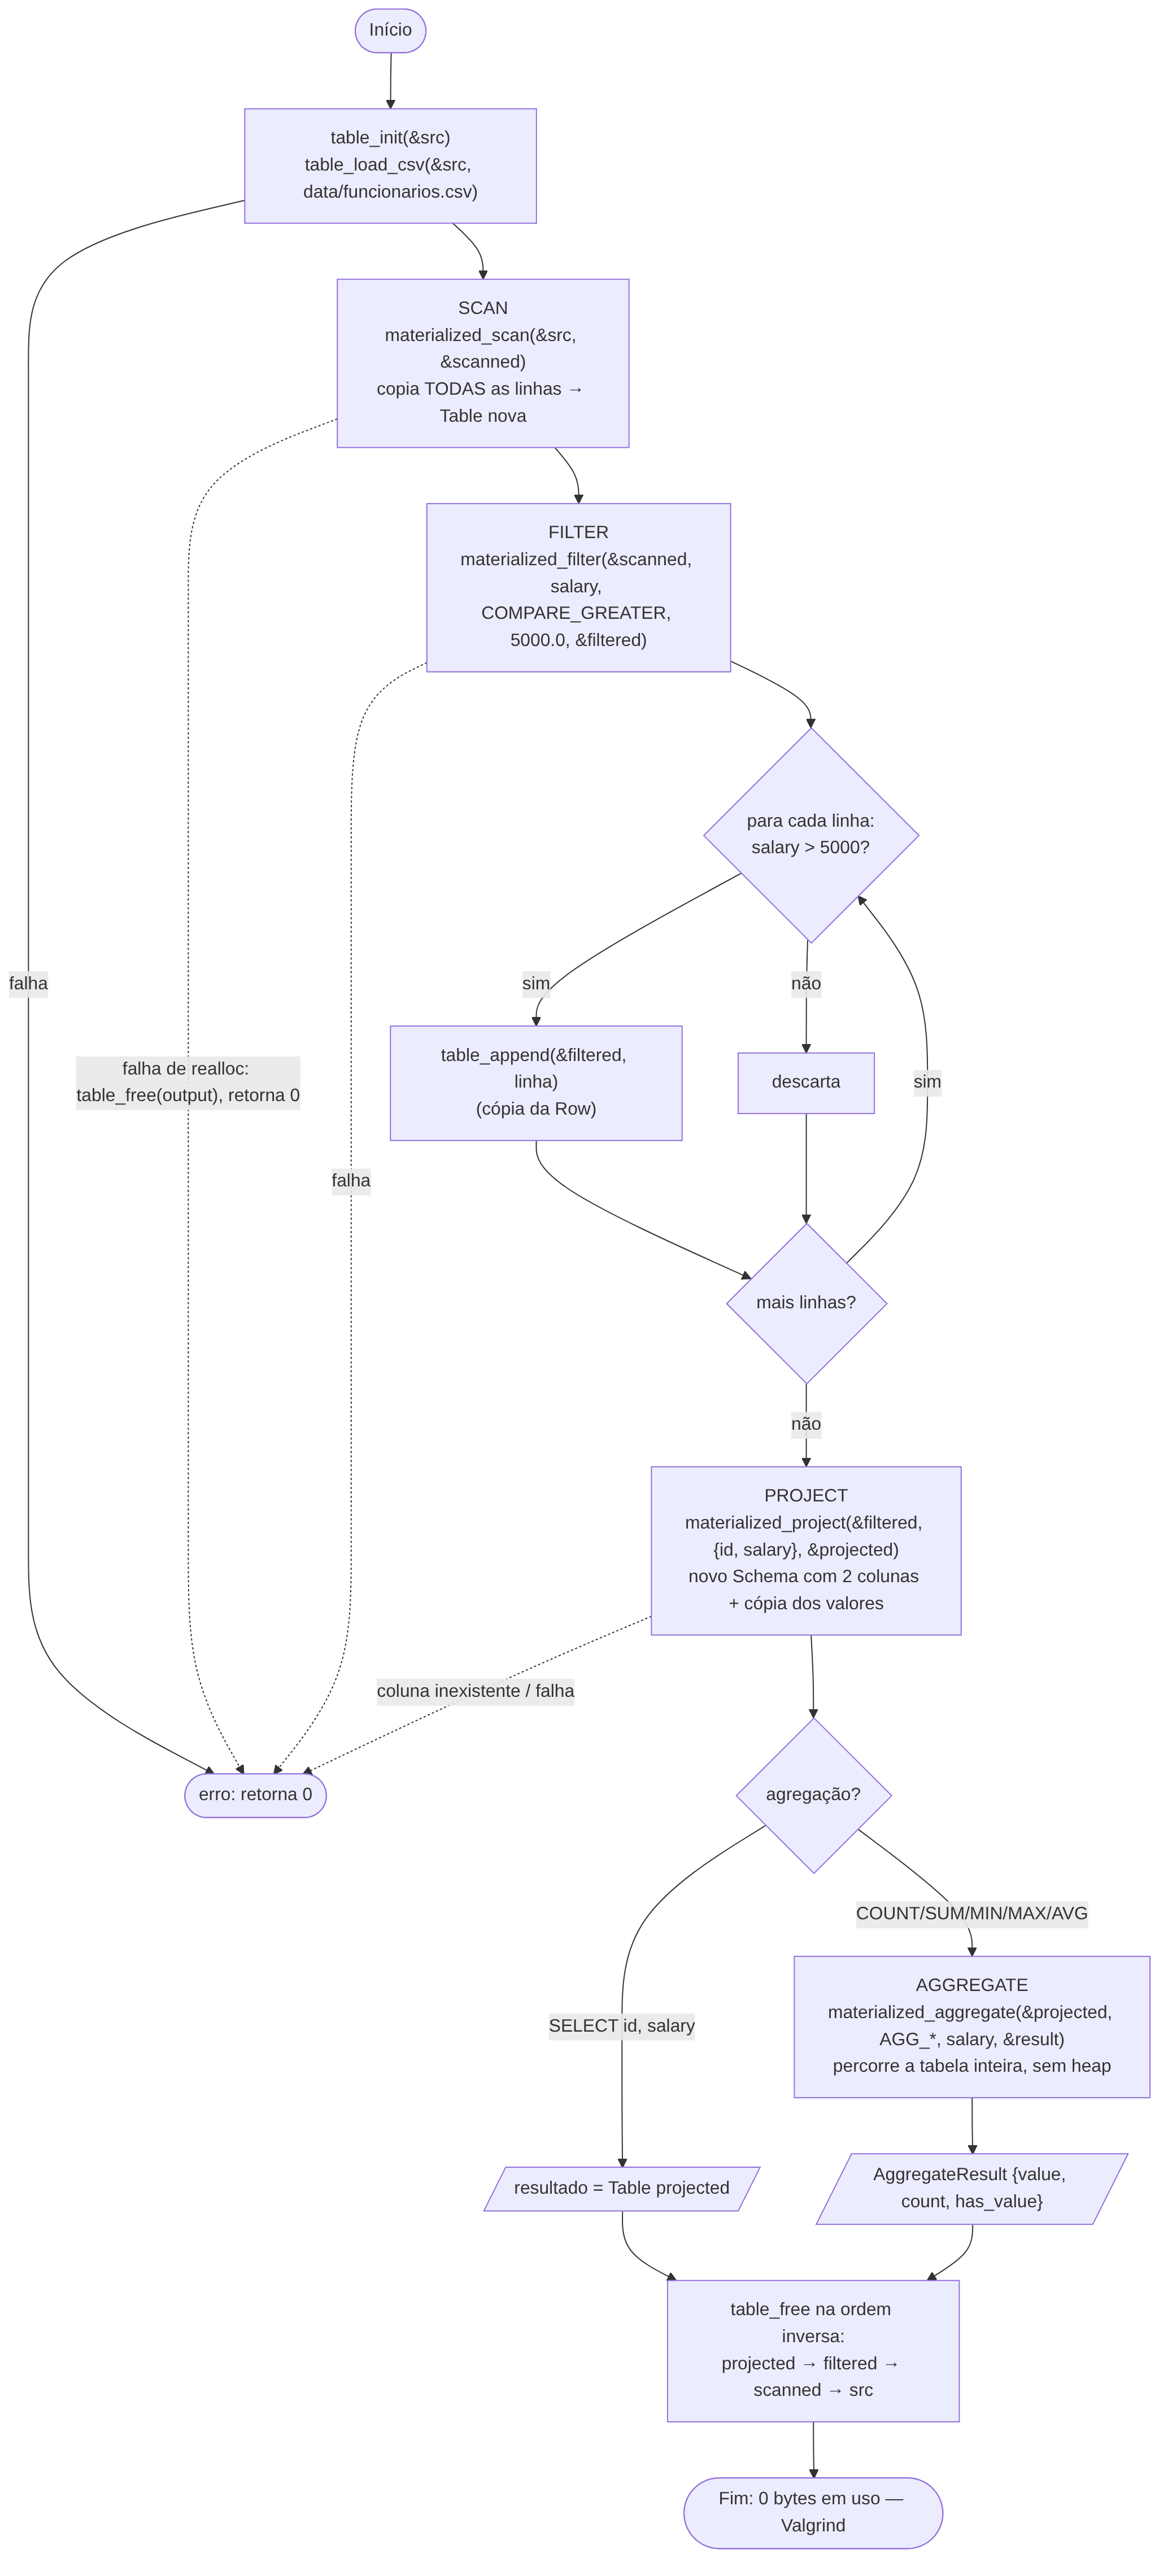
\includegraphics[height=0.88\textheight,keepaspectratio]{fluxograma.png}
\caption{Fluxograma do pipeline materializado da etapa 2.}
\label{fig:fluxo}
\end{figure}

\section{Testes}
\texttt{make test} compila a suíte com \texttt{-std=c11 -Wall -Wextra -Wpedantic -Werror -O2} e termina com \texttt{all materialized tests passed}. Para a etapa 2, os testes cobrem a leitura do CSV e o esquema, a independência da cópia do SCAN, os limites e erros do FILTER, a projeção ordenada e seus casos de erro, cada agregação (inclusive em tabela vazia) e o pipeline completo.

\section{Dificuldades encontradas}
\begin{itemize}
    \item \textbf{Linha de tamanho fixo.} A estrutura anterior usava uma linha fixa de funcionário (\texttt{EmployeeRow}), o que impedia projetar colunas em outra ordem ou com esquema menor. Ela foi substituída por \texttt{Schema} e \texttt{Row}/\texttt{Value} tipados, com esquema variável por tabela, mantendo o formato do CSV.
    \item \textbf{Propriedade das strings.} Ponteiros para o buffer de leitura do CSV ficariam inválidos e strings alocadas por célula aumentariam o risco de vazamento. A solução foi embutir as strings no \texttt{Value}, ao custo de um limite de 127 caracteres por valor e de mais memória por linha.
    \item \textbf{Valor esperado no teste.} O valor esperado da média no teste do pipeline foi corrigido para $22\,800 / 3 = 7600$, que é a média dos três salários filtrados.
    \item \textbf{Ambiente de validação.} A validação de memória com Valgrind, AddressSanitizer e UBSan foi feita em Linux, com os resultados da Seção~\ref{sec:valgrind}.
    \item \textbf{FILTER sensível a tipo.} Comparar \texttt{salary} (\texttt{DOUBLE}) com um inteiro é rejeitado. Isso foi mantido como decisão de projeto: o chamador usa \texttt{value\_double(5000.0)}.
\end{itemize}

\section{Possíveis otimizações}
As otimizações a seguir partem de limitações reais do código atual.
\begin{enumerate}
    \item \textbf{Liberar cada intermediário assim que o consumidor termina.} Hoje, no teste do pipeline, todas as tabelas ficam vivas até o fim, e o pico de memória é a soma de fonte, SCAN, FILTER e PROJECT. Liberando cada uma logo depois do operador seguinte, o pico cairia para cerca de duas tabelas.
    \item \textbf{SCAN sem cópia ou fundido com o FILTER.} O SCAN duplica a tabela inteira. Eliminar essa cópia economiza memória, mas deixa de ser uma materialização pura.
    \item \textbf{Linha compacta.} Cada \texttt{Row} reserva 16 valores de 136 bytes (2176 bytes), mesmo com 2 colunas. Alocando só as colunas do esquema, a tabela projetada \texttt{id, salary} usaria cerca de 32 bytes de dados por linha.
    \item \textbf{Strings fora da linha.} Um pool ou arena de strings de tamanho variável reduziria a memória, desde que se defina claramente o dono e a liberação.
    \item \textbf{Armazenamento colunar.} PROJECT e AGGREGATE leriam só as colunas usadas, com melhor aproveitamento de cache.
    \item \textbf{Capacidade exata.} SCAN e PROJECT conhecem \texttt{input->size} de antemão e poderiam reservar o vetor uma única vez, sem \texttt{realloc} repetidos nem capacidade sobrando.
    \item \textbf{Arena por consulta.} Todas as tabelas de uma consulta seriam liberadas de uma vez, com menos fragmentação.
    \item \textbf{Fusão de FILTER e PROJECT e predicados compostos.} Menos passagens pelos dados, aproximando a execução do modelo pipeline \cite{graefe}.
    \item \textbf{Medição de tempo de parede com repetições.} \texttt{clock()} mede tempo de CPU e fica perto de zero com 6 linhas. Benchmarks confiáveis precisam de várias execuções e da mediana.
    \item \textbf{Leitor de CSV mais robusto.} \texttt{table\_load\_csv} ignora o cabeçalho e separa campos com \texttt{strtok}. Validar o cabeçalho contra o esquema e tratar aspas e valores nulos evitaria erros de dados.
\end{enumerate}

\section{Conclusão}
A etapa 2 implementa o pipeline SCAN $\rightarrow$ FILTER $\rightarrow$ PROJECT $\rightarrow$ AGGREGATE no modelo materializado, com cada operador produzindo uma tabela própria e independente. A projeção \texttt{SELECT id, salary WHERE salary > 5000} retorna as 3 linhas esperadas, e as cinco agregações produzem valores coerentes com os dados. A posse da memória é simples: um único vetor de heap por tabela, liberado pelo chamador, com liberação da saída parcial em todo caminho de erro. A validação com Valgrind terminou com 81 alocações, 81 liberações, nenhum vazamento e nenhum erro.

{\small
\begin{thebibliography}{9}
\bibitem{graefe}
G. Graefe.
\newblock Query evaluation techniques for large databases.
\newblock \emph{ACM Computing Surveys}, 25(2):73--169, 1993.

\bibitem{garcia}
H. Garcia-Molina, J. D. Ullman e J. Widom.
\newblock \emph{Database Systems: The Complete Book}.
\newblock 2.\ ed. Pearson Prentice Hall, 2008.

\bibitem{valgrind}
Valgrind Developers.
\newblock \emph{Valgrind User Manual -- Memcheck: a memory error detector}.
\newblock Disponível em: \url{https://valgrind.org/docs/manual/mc-manual.html}.
\end{thebibliography}
}

\end{document}
